\section{Electronic Components}

\subsection{Sensors and Analogue Circuit}

\begin{figure}[H]
    \centering
    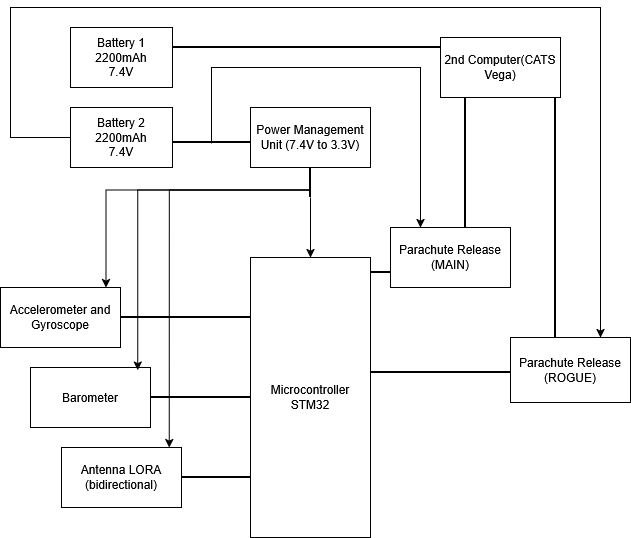
\includegraphics[width=0.85\linewidth]{Images/2_eletronic_components/eletrical_diagram.png}
    \caption{Electrical system diagram}
    \label{fig:electrical_diagram}
\end{figure}

\subsubsection{Battery System}

The avionics system is powered by Lithium-Polymer (LiPo) batteries. The primary battery used for the SRAD electronics is a Gens Ace 2S1P LiPo battery rated at 7.4\,V nominal voltage and 2400\,mAh capacity. The battery features a two-cell configuration and a 30C discharge rating, providing sufficient current capability for all avionics loads while maintaining minimal voltage sag. An XT60 connector is used to ensure a reliable and low-resistance power connection.

This battery was selected due to its high energy density, low mass, and robust discharge performance.

A second independent battery powers the COTS flight computer, ensuring redundancy in the event of a failure in the primary avionics power system.

\begin{itemize}
    \item \textbf{Main Battery (SRAD):} 7.4\,V, 2400\,mAh
    \item \textbf{Redundancy Battery (COTS Flight Computer):} 7.4\,V, 2400\,mAh
\end{itemize}

Additionally, external power can be supplied through a pad connector during pre-flight operations, allowing the onboard batteries to remain fully charged until launch.

\begin{table}[H]
\centering
\begin{tabular}{|l|l|}
\hline
\textbf{Parameter} & \textbf{Value} \\ \hline
Balancer Connector Type & JST-XHR-2P \\ \hline
Brand & Gens Ace \\ \hline
Capacity (mAh) & 2400 \\ \hline
Voltage (V) & 7.4 \\ \hline
Length (±5mm) & 88 \\ \hline
Width (±2mm) & 29 \\ \hline
Height (±2mm) & 17 \\ \hline
Net Weight (±20g) & 94 \\ \hline
\end{tabular}
\caption{Specifications of the Gens Ace 7.4V 2400mAh LiPo battery}
\label{tab:gensace2400}
\end{table}

\subsubsection{Power Management Unit (PMU)}

The Power Management Unit (PMU) is responsible for regulating and distributing power to the onboard electronics. Instead of using a simple voltage divider, the system employs an LT317A voltage regulator to provide a stable 3.3\,V output under varying current loads.

The PMU converts the main battery voltage into regulated 5\,V and 3.3\,V supply rails required by the avionics systems. For safety purposes, the PMU can be disconnected through an arming pin during handling and integration procedures.

\begin{figure}[H]
    \centering
    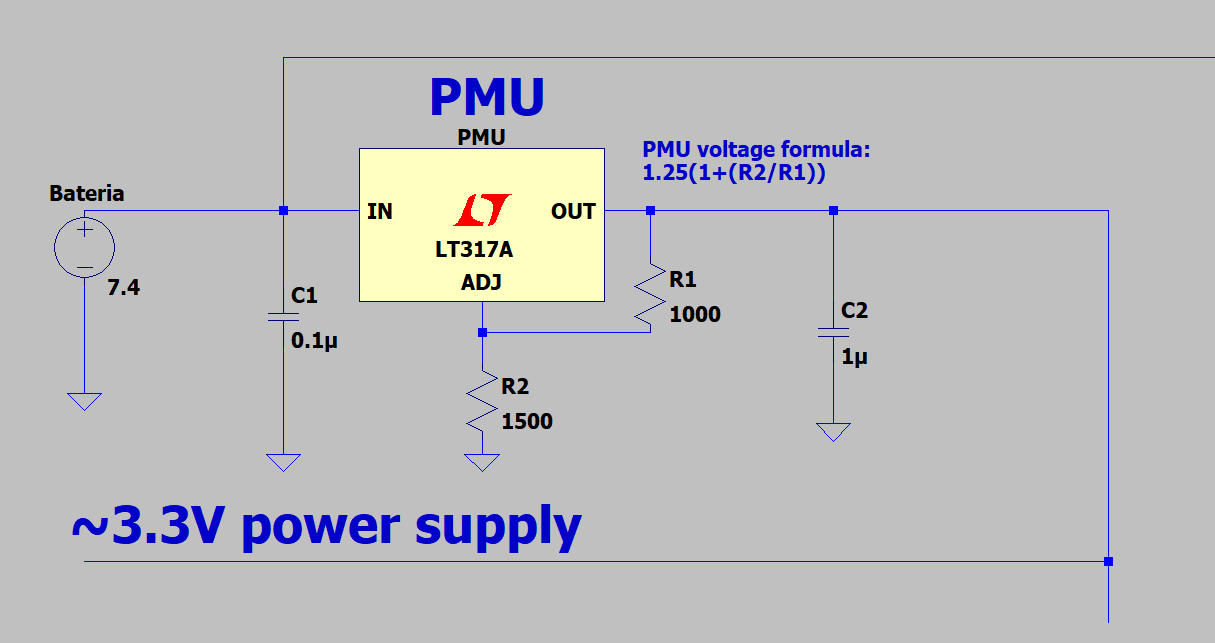
\includegraphics[width=0.85\linewidth]{Images/2_eletronic_components/PMU.png}
    \caption{Power Management Unit schematic}
    \label{fig:pmu}
\end{figure}

\subsubsection{Sensors}

\paragraph{MPU6050 -- Gyroscope and Accelerometer}

The MPU6050 is a 6-degree-of-freedom (6-DOF) Inertial Measurement Unit (IMU) integrating a 3-axis MEMS gyroscope and a 3-axis MEMS accelerometer on a single chip. The sensor communicates through the I\textsuperscript{2}C protocol and incorporates 16-bit Analog-to-Digital Converters (ADCs), allowing precise motion tracking and orientation estimation in high-dynamic environments.

\paragraph{Pin Description}

\begin{itemize}
    \item \textbf{INT} -- Interrupt digital output pin
    \item \textbf{AD0} -- I\textsuperscript{2}C slave address least significant bit pin
    \item \textbf{XCL} -- Auxiliary serial clock pin
    \item \textbf{XDA} -- Auxiliary serial data pin
    \item \textbf{SDA} -- Serial data pin
    \item \textbf{SCL} -- Serial clock pin
    \item \textbf{GND} -- Ground reference (0\,V)
    \item \textbf{VCC} -- Power supply input (+3.3\,V)
\end{itemize}

\paragraph{Sensitivity Scale Factors}

To convert the raw digital sensor output into physical units, the measured values are divided by the sensitivity scale factor corresponding to the selected full-scale range.

\begin{center}
\begin{tabular}{ccc}
\toprule
\textbf{Full-Scale Range} & \textbf{Accelerometer Sensitivity} & \textbf{Gyroscope Sensitivity} \\
\midrule
$\pm2g$ / $\pm250^\circ$/s & 16384 LSB/g & 131 LSB/($^\circ$/s) \\
$\pm4g$ / $\pm500^\circ$/s & 8192 LSB/g & 65.5 LSB/($^\circ$/s) \\
$\pm8g$ / $\pm1000^\circ$/s & 4096 LSB/g & 32.8 LSB/($^\circ$/s) \\
$\pm16g$ / $\pm2000^\circ$/s & 2048 LSB/g & 16.4 LSB/($^\circ$/s) \\
\bottomrule
\end{tabular}
\end{center}

\paragraph{Accelerometer Calculations}

The accelerometer output is represented as a signed 16-bit integer ranging from $-32768$ to $32767$. For this project, the $\pm16g$ full-scale range is selected.

Velocity is obtained by integrating acceleration over time using the trapezoidal method for discrete time intervals $\Delta t$.

\paragraph{Gyroscope Calculations}

At the $\pm2000^\circ$/s full-scale setting, angular velocity is obtained by dividing the raw sensor value by the corresponding sensitivity factor.

Angular position is estimated through numerical integration of the angular velocity over time.

\subsubsection{Parachute Release System}

The recovery system consists of two independent parachute deployment mechanisms: a drogue parachute and a main parachute.

The STM32 flight computer controls the deployment sequence using sensor data and onboard flight algorithms. For the main parachute, the STM32 activates a transistor that allows high current from the battery to pass through a low-impedance resistor. The resulting heat ignites a pyrotechnic compound that burns the restraining cable and releases the parachute.

As a redundancy measure, the CATS Vega flight computer can independently trigger deployment through a separate transistor in the event of an STM32 failure.

The drogue parachute is deployed using a servo-actuated latch mechanism. The servo releases the latch, which in turn deploys the drogue parachute and subsequently enables safe deployment of the main parachute.

\begin{figure}[H]
    \centering
    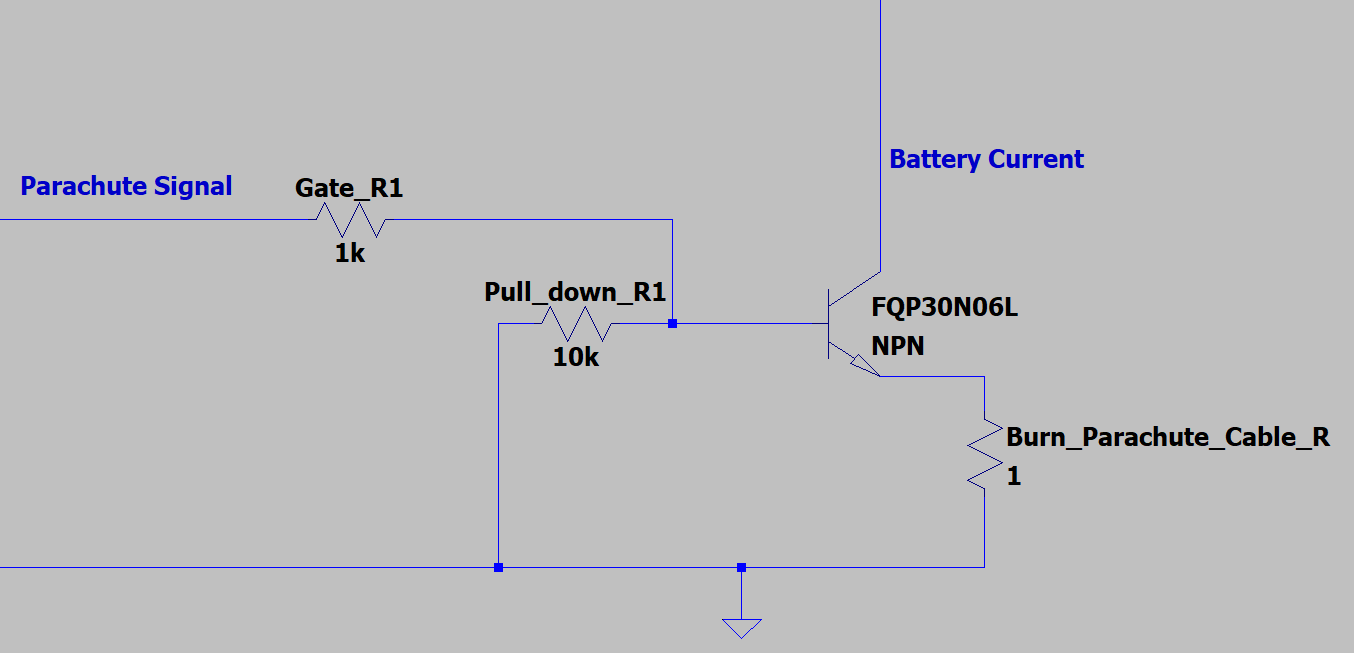
\includegraphics[width=0.85\linewidth]{Images/2_eletronic_components/main_parachute_eletrical_diagram.png}
    \caption{Main parachute electrical diagram}
    \label{fig:main_parachute}
\end{figure}

\begin{figure}[H]
    \centering
    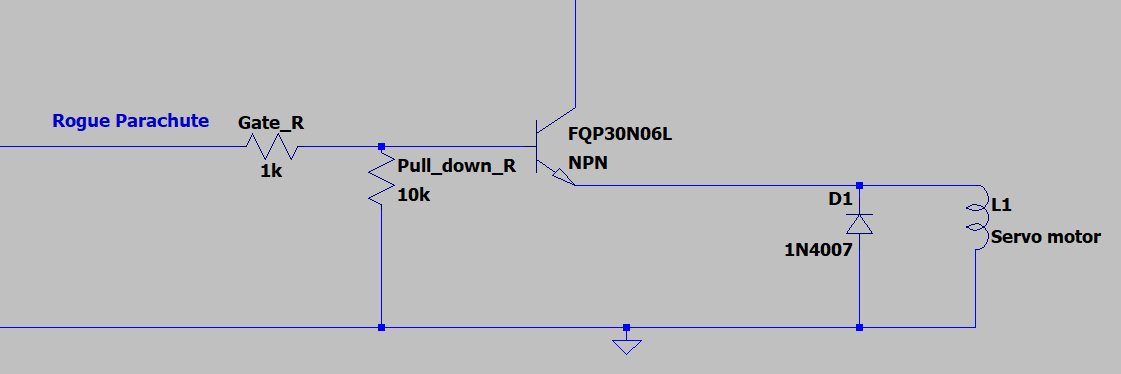
\includegraphics[width=0.85\linewidth]{Images/2_eletronic_components/rogue_parachute_eletrical_diagram.png}
    \caption{Drogue parachute electrical diagram}
    \label{fig:drogue_parachute}
\end{figure}
